\documentclass[12pt, a4paper]{ctexart}
\usepackage{geometry}
\geometry{left=2.5cm, right=2.5cm, top=3cm, bottom=3cm}
\usepackage{graphicx}
\usepackage{xcolor}
\usepackage{circuitikz}
\usepackage{subcaption}
\usepackage{float}
\usepackage{amsmath}
\usetikzlibrary{arrows, shapes.gates.logic.US, positioning}
\tikzset{
    dot/.style={circle, fill, inner sep=1pt}
}
\ctikzset{
    logic ports=ieee,
    logic ports/scale=0.8
}

\begin{document}

% 封面
\begin{titlepage}
    \centering
    \vspace*{5cm}
    {\Huge\bfseries 实验报告\par}
    \vspace{2cm}
    {\Large 课程：数字逻辑与计算机组成\par}
    \vspace{1cm}
    {\Large 实验一：基本逻辑部件设计\par}
    \vspace{4cm}
    {\large 姓名：\underline{\makebox[4cm]{郑袭明}}\par}
    \vspace{1cm}
    {\large 学号：\underline{\makebox[4cm]{251502027}}\par}
    \vspace{1cm}
    {\large 日期：\today\par}
\end{titlepage}

\tableofcontents
\newpage

\section{实验目的}

\begin{enumerate}
    \item 掌握 Logisim 软件的使用方法和实验步骤。
    \item 掌握 CMOS 晶体管的特性以及逻辑门电路的构建法。
    \item 掌握使用不同组件实现多路选择器的设计方法。
    \item 掌握电路外观设计方法。
    \item 掌握子电路级联设计方法。
\end{enumerate}

\section{实验一：多数表决器实验}

\subsection{整体方案设计}

功能：当输入 X、Y、Z 中至少有两个为 1 时，输出 F 为 1，否则输出 F 为 0。

表达式：$F = XY + XZ + YZ$

\begin{table}[H]
    \centering
    \begin{tabular}{|c|c|}
        \hline
        引脚 & 功能 \\
        \hline
        X & 输入 \\
        Y & 输入 \\
        Z & 输入 \\
        F & 输出 \\
        \hline
    \end{tabular}
    \caption{多数表决器引脚功能表}
\end{table}

\subsection{电路设计}

\begin{figure}[H]
    \centering
    \subcaptionbox{原理图}{
        \begin{circuitikz}
            \node[muxdemux,
                muxdemux def={Lh=4, Rh=4, NL=3, NB=0}
            ] (mux) {};
            \node[left] (X) at (mux.lpin 1) {X};
            \node[left] (Y) at (mux.lpin 2) {Y};
            \node[left] (Z) at (mux.lpin 3) {Z};
            \node[right] (F) at (mux.rpin 1) {F};
        \end{circuitikz}
    }
    \subcaptionbox{电路图}{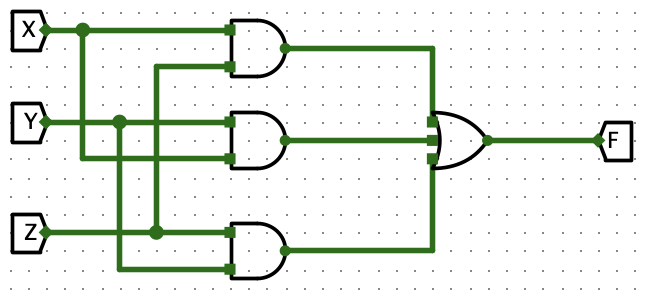
\includegraphics[width=0.4\textwidth]{assets/exp1/circuit.png}}
    \caption{多数表决器电路设计}
\end{figure}

\subsection{仿真结果}

\begin{figure}[H]
    \centering
    \subcaptionbox{}{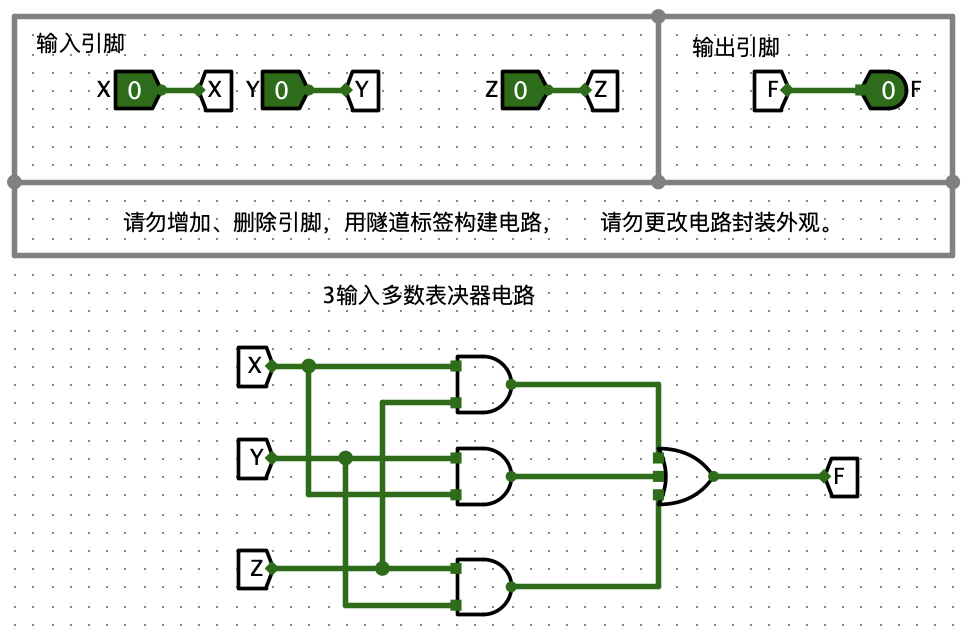
\includegraphics[width=0.4\textwidth]{assets/exp1/sim1.png}}
    \subcaptionbox{}{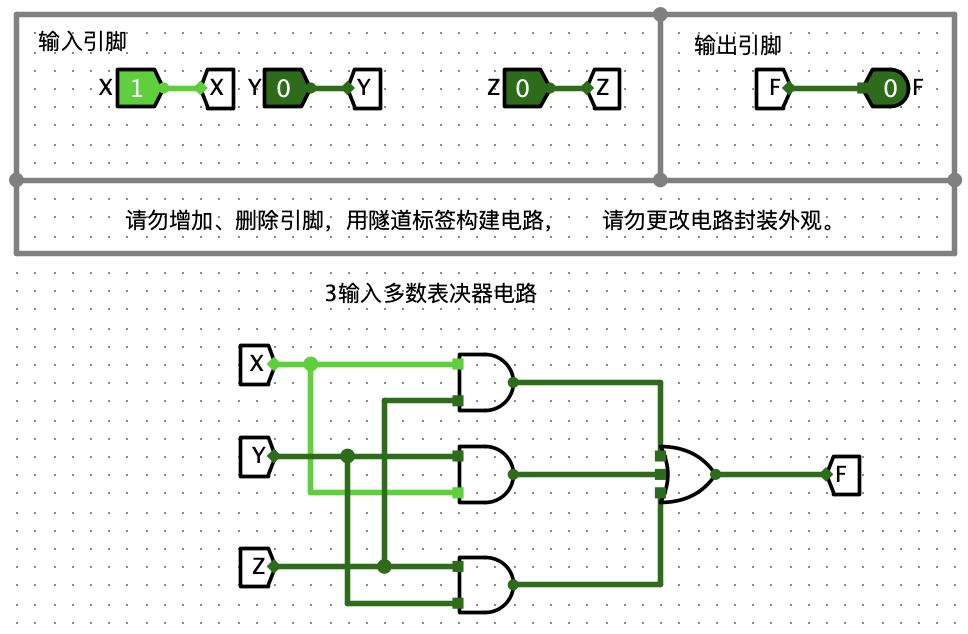
\includegraphics[width=0.4\textwidth]{assets/exp1/sim2.png}}
    \subcaptionbox{}{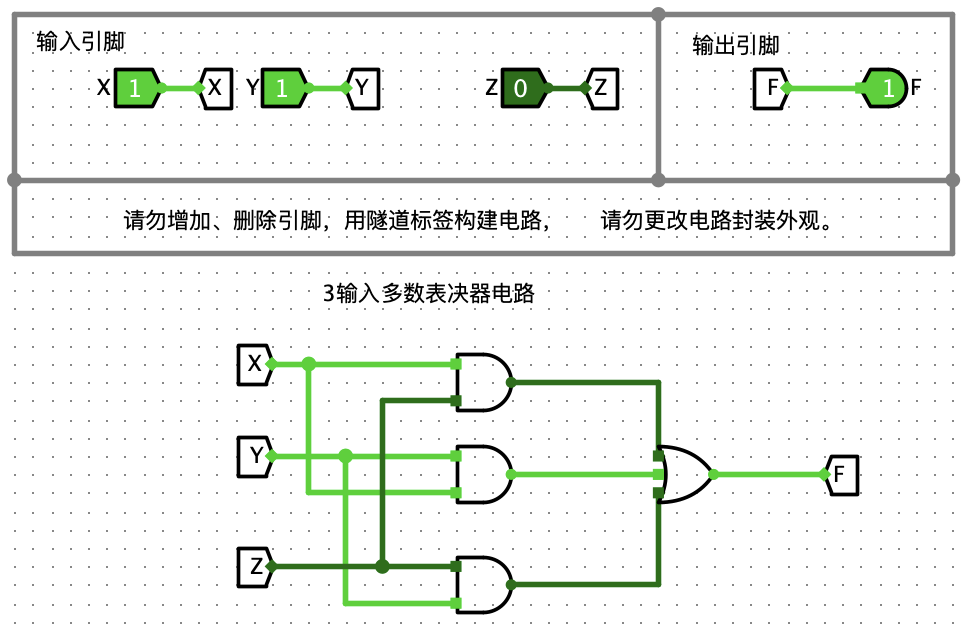
\includegraphics[width=0.4\textwidth]{assets/exp1/sim3.png}}
    \subcaptionbox{}{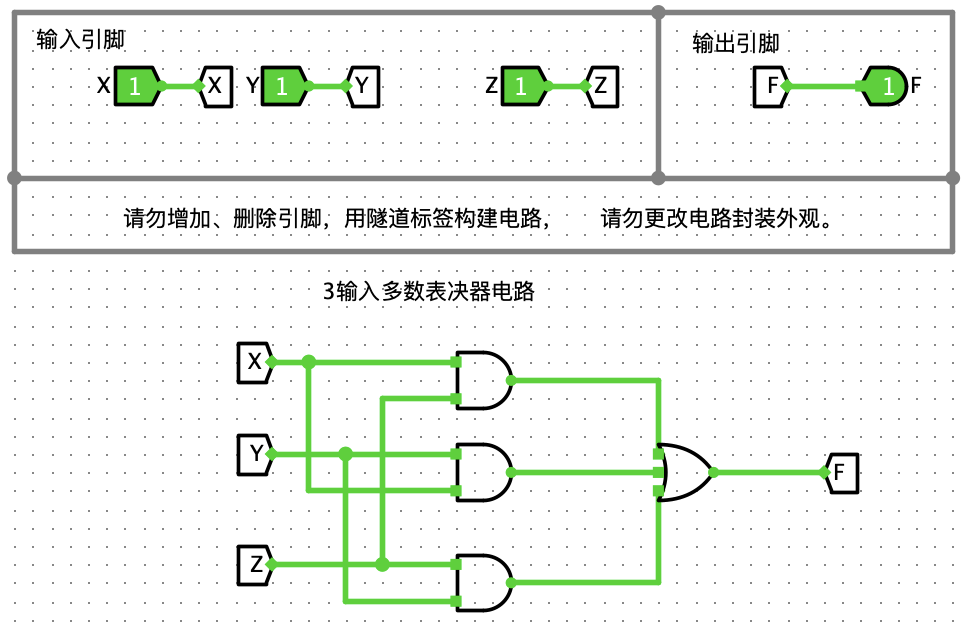
\includegraphics[width=0.4\textwidth]{assets/exp1/sim4.png}}
    \caption{多数表决器仿真结果}
\end{figure}

\begin{table}[H]
    \centering
    \begin{tabular}{|c|c|c|c|}
        \hline
        X & Y & Z & F \\
        \hline
        0 & 0 & 0 & 0 \\
        0 & 0 & 1 & 0 \\
        0 & 1 & 0 & 0 \\
        0 & 1 & 1 & 1 \\
        1 & 0 & 0 & 0 \\
        1 & 0 & 1 & 1 \\
        1 & 1 & 0 & 1 \\
        1 & 1 & 1 & 1 \\
        \hline
    \end{tabular}
    \caption{多数表决器真值表}
\end{table}

\subsection{错误现象及分析}

在完成实验的过程中，没有遇到任何错误。

\section{实验二：晶体管构建或门实验}

\subsection{整体方案设计}

利用 CMOS 晶体管构建两输入或门。

基本原理：根据数字电路原理，或门是由或非门级联反相器构成。

\begin{table}[H]
    \centering
    \begin{tabular}{|c|c|}
        \hline
        引脚 & 功能 \\
        \hline
        A & 输入 \\
        B & 输入 \\
        F & 输出 \\
        \hline
    \end{tabular}
    \caption{晶体管构建或门引脚功能表}
\end{table}

\subsection{电路设计}

\begin{figure}[H]
    \centering
    \subcaptionbox{原理图}{
        \begin{circuitikz}
            \node[nor port, number inputs=2] (nor) at (0,0) {};
            \node[left] (A) at (nor.in 1) {A};
            \node[left] (B) at (nor.in 2) {B};
            \node[not gate US, draw] (not) at (1.5,0) {};
            \node[right] (F) at (2,0) {F};
            \draw (nor.out) -- (not.input);
            \draw (not.output) -- (F);
        \end{circuitikz}
    }
    \subcaptionbox{电路图}{
\includegraphics[width=0.6\textwidth]{assets/exp2/circuit.png}}
    \caption{晶体管构建或门电路设计}
\end{figure}

\subsection{仿真结果}

\begin{figure}[H]
    \centering
    \subcaptionbox{}{
\includegraphics[width=0.4\textwidth]{assets/exp2/sim1.png}}
    \subcaptionbox{}{
\includegraphics[width=0.4\textwidth]{assets/exp2/sim2.png}}
    \subcaptionbox{}{
\includegraphics[width=0.4\textwidth]{assets/exp2/sim3.png}}
    \subcaptionbox{}{
\includegraphics[width=0.4\textwidth]{assets/exp2/sim4.png}}
    \caption{晶体管构建或门仿真结果}
\end{figure}

\begin{table}[H]
    \centering
    \begin{tabular}{|c|c|c|}
        \hline
        A & B & F \\
        \hline
        0 & 0 & 0 \\
        0 & 1 & 1 \\
        1 & 0 & 1 \\
        1 & 1 & 1 \\
        \hline
    \end{tabular}
    \caption{晶体管构建或门真值表}
\end{table}

\subsection{错误现象及分析}

进行实验时，晶体管的朝向错误，导致电路无法正常工作。通过检查电路图，发现晶体管的源极和漏极连接反了，调整后电路正常工作。

\begin{figure}[H]
    \centering
    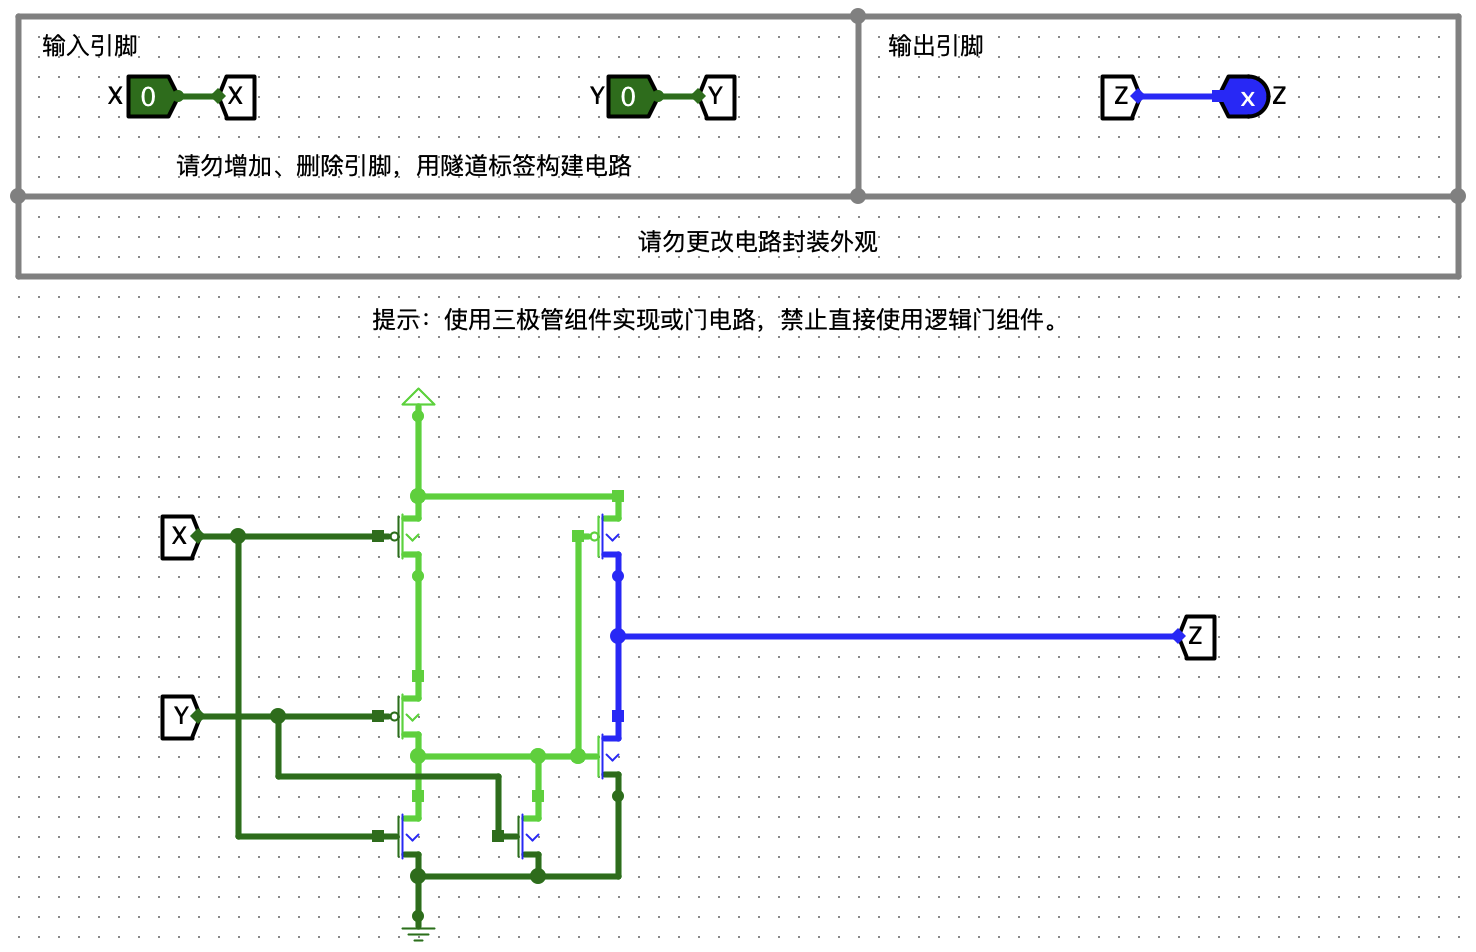
\includegraphics[width=0.5\textwidth]{assets/exp2/error.png}
    \caption{晶体管朝向错误导致的电路问题}
\end{figure}

\section{实验三：2 选 1 多路选择器实验1}

\subsection{整体方案设计}

利用基本逻辑部件，实现 2 选 1 多路选择器。

\begin{table}[H]
    \centering
    \begin{tabular}{|c|c|}
        \hline
        引脚 & 功能 \\
        \hline
        D0 & 输入0 \\
        D1 & 输入1 \\
        S & 选择信号 \\
        Y & 输出 \\
        \hline
    \end{tabular}
    \caption{2 选 1 多路选择器引脚功能表}
\end{table}

\subsection{电路设计}

\begin{figure}[H]
    \centering
    \subcaptionbox{原理图}{
        \begin{circuitikz}
            \node[muxdemux,
                muxdemux def={Lh=4, Rh=2, NL=2, NB=1},
                muxdemux label={L1=0,L2=1}
            ] (mux) {MUX};
            \node[left] (D0) at (mux.lpin 1) {D0};
            \node[left] (D1) at (mux.lpin 2) {D1};
            \node[below] (S) at (mux.bpin 1) {S};
            \node[right] (Y) at (mux.rpin 1) {Y};
        \end{circuitikz}
    }
    \subcaptionbox{电路图}{
\includegraphics[width=0.5\textwidth]{assets/exp3/circuit.png}}
    \caption{2 选 1 多路选择器电路设计}
\end{figure}

\subsection{仿真结果}

\begin{figure}[H]
    \centering
    \subcaptionbox{}{
\includegraphics[width=0.4\textwidth]{assets/exp3/sim1.png}}
    \subcaptionbox{}{
\includegraphics[width=0.4\textwidth]{assets/exp3/sim2.png}}
    \caption{2 选 1 多路选择器仿真结果}
\end{figure}

\begin{table}[H]
    \centering
    \begin{tabular}{|c|c|c|}
        \hline
        D0 & D1 & Y \\
        \hline
        0 & 0 & 0 \\
        0 & 1 & 0 \\
        1 & 0 & 1 \\
        1 & 1 & 1 \\
        \hline
    \end{tabular}
    \caption{2 选 1 多路选择器真值表}
\end{table}

\subsection{错误现象及分析}

在完成实验的过程中，没有遇到任何错误。

\section{实验四：2 选 1 多路选择器实验2}

\subsection{整体方案设计}

利用晶体管和传输门，实现 2 选 1 多路选择器。

\begin{table}[H]
    \centering
    \begin{tabular}{|c|c|}
        \hline
        引脚 & 功能 \\
        \hline
        D0 & 输入0 \\
        D1 & 输入1 \\
        S & 选择信号 \\
        Y & 输出 \\
        \hline
    \end{tabular}
    \caption{2 选 1 多路选择器引脚功能表}
\end{table}

\subsection{电路设计}

原理与实验三相同，但电路实现方式不同，使用晶体管和传输门来实现多路选择器的功能。

\begin{figure}[H]
    \centering
    \subcaptionbox{原理图}{
        \begin{circuitikz}
            \node[muxdemux,
                muxdemux def={Lh=4, Rh=2, NL=2, NB=1},
                muxdemux label={L1=0,L2=1}
            ] (mux) {MUX};
            \node[left] (D0) at (mux.lpin 1) {D0};
            \node[left] (D1) at (mux.lpin 2) {D1};
            \node[below] (S) at (mux.bpin 1) {S};
            \node[right] (Y) at (mux.rpin 1) {Y};
        \end{circuitikz}
    }
    \subcaptionbox{电路图}{
\includegraphics[width=0.5\textwidth]{assets/exp4/circuit.png}}
    \caption{2 选 1 多路选择器电路设计}
\end{figure}

\subsection{仿真结果}

\begin{figure}[H]
    \centering
    \subcaptionbox{}{
\includegraphics[width=0.4\textwidth]{assets/exp4/sim1.png}}
    \subcaptionbox{}{
\includegraphics[width=0.4\textwidth]{assets/exp4/sim2.png}}
    \caption{2 选 1 多路选择器仿真结果}
\end{figure}

\begin{table}[H]
    \centering
    \begin{tabular}{|c|c|c|}
        \hline
        D0 & D1 & Y \\
        \hline
        0 & 0 & 0 \\
        0 & 1 & 0 \\
        1 & 0 & 1 \\
        1 & 1 & 1 \\
        \hline
    \end{tabular}
    \caption{2 选 1 多路选择器真值表}
\end{table}

\subsection{错误现象及分析}

在完成实验的过程中，没有遇到任何错误。

\section{实验五：4 选 1 多路选择器实验}

\subsection{整体方案设计}

封装上一实验实现的 2 选 1 多路选择器，实现 4 选 1 多路选择器。

\begin{figure}[H]
    \centering
    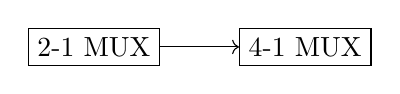
\begin{tikzpicture}
        \node[draw] (2-1mux) {2-1 MUX};
        \node[draw, right=of 2-1mux] (4-1mux) {4-1 MUX};
        \draw[->] (2-1mux) -- (4-1mux);
    \end{tikzpicture}
    \caption{4 选 1 多路选择器设计思路}
\end{figure}

\begin{table}[H]
    \centering
    \begin{tabular}{|c|c|}
        \hline
        引脚 & 功能 \\
        \hline
        D0 & 输入0 \\
        D1 & 输入1 \\
        D2 & 输入2 \\
        D3 & 输入3 \\
        S0 & 选择信号0 \\
        S1 & 选择信号1 \\
        Y & 输出 \\
        \hline
    \end{tabular}
    \caption{4 选 1 多路选择器引脚功能表}
\end{table}

\subsection{电路设计}

\begin{figure}[H]
    \centering
    \subcaptionbox{原理图}{
        \begin{circuitikz}
            \node[muxdemux,
                muxdemux def={Lh=4, Rh=2, NL=4, NB=2},
                muxdemux label={L1=00,L2=01,L3=10,L4=11}
            ] (mux) {MUX};
            \node[left] (D0) at (mux.lpin 1) {D0};
            \node[left] (D1) at (mux.lpin 2) {D1};
            \node[left] (D2) at (mux.lpin 3) {D2};
            \node[left] (D3) at (mux.lpin 4) {D3};
            \node[below] (S0) at (mux.bpin 2) {S0};
            \node[below] (S1) at (mux.bpin 1) {S1};
            \node[right] (Y) at (mux.rpin 1) {Y};
        \end{circuitikz}
    }
    \subcaptionbox{电路图}{
\includegraphics[width=0.5\textwidth]{assets/exp5/circuit.png}}
    \caption{4 选 1 多路选择器电路设计}
\end{figure}

\subsection{仿真结果}

\begin{figure}[H]
    \centering
    \subcaptionbox{}{
\includegraphics[width=0.4\textwidth]{assets/exp5/sim1.png}}
    \subcaptionbox{}{
\includegraphics[width=0.4\textwidth]{assets/exp5/sim2.png}}
    \subcaptionbox{}{
\includegraphics[width=0.4\textwidth]{assets/exp5/sim3.png}}
    \subcaptionbox{}{
\includegraphics[width=0.4\textwidth]{assets/exp5/sim4.png}}
    \caption{4 选 1 多路选择器仿真结果}
\end{figure}

\begin{table}[H]
    \centering
    \begin{tabular}{|c|c|c|}
        \hline
        S1 & S0 & Y \\
        \hline
        0 & 0 & D0 \\
        0 & 1 & D1 \\
        1 & 0 & D2 \\
        1 & 1 & D3 \\
        \hline
    \end{tabular}
    \caption{4选1多路选择器真值表}
\end{table}

\subsection{错误现象及分析}

在完成实验的过程中，没有遇到任何错误。

\section{思考题}

\subsection{2 选 1 多路选择器的与非-与非电路}

由表达式

\begin{equation}
    \begin{aligned}
        Y &= D_0\overline{S}+D_1S
        \\&= \overline{\overline{D_0\overline{S}}\cdot\overline{D_1\cdot S}}
    \end{aligned}
\end{equation}

可画出电路图

\begin{figure}[H]
    \centering
    \begin{circuitikz}
        \node[nand gate US, draw, logic gate inputs=ni] (nand1) at (2,0) {};
        \node[nand gate US, draw, logic gate inputs=nn] (nand2) at (2,-1) {};
        \node[left] (D0) at (0,0 |- nand1.input 1) {D0};
        \node[left] (D1) at (0,0 |- nand2.input 1) {D1};
        \node[left] (S) at (0,-2) {S};
        \node[nand gate US, draw] (nand3) at (4,-0.5) {};
        \node[right] (Y) at (5,-0.5) {Y};
        \draw (D0) -- (nand1.input 1);
        \draw (S) -- (1,-2) |- (nand1.input 2);
        \draw (D1) -- (nand2.input 1);
        \draw (S) -- (1,-2) |- node[dot]{} (nand2.input 2);
        \draw (nand1.output) -- (3,0) |- (nand3.input 1);
        \draw (nand2.output) -- (3,-1) |- (nand3.input 2);
        \draw (nand3.output) -- (Y);
    \end{circuitikz}
    \caption{2 选 1 多路选择器的与非-与非电路}
\end{figure}

\subsection{4 位二进制数转换成格雷码的转换电路}

由表达式

\begin{equation}
    \begin{aligned}
        G_3 &= B_3
        \\G_2 &= B_3 \oplus B_2
        \\G_1 &= B_2 \oplus B_1
        \\G_0 &= B_1 \oplus B_0
    \end{aligned}
\end{equation}

可画出电路图

\begin{figure}[H]
    \centering
    \begin{circuitikz}
        \node[xor gate US, draw, logic gate inputs=nn] (xor1) at (0,0) {};
        \node[xor gate US, draw, logic gate inputs=nn] (xor2) at (0,-1) {};
        \node[xor gate US, draw, logic gate inputs=nn] (xor3) at (0,-2) {};
        \node[left] (B3) at (-1.5,1) {B3};
        \node[left] (B2) at (-1.5,0 |- xor1.input 2) {B2};
        \node[left] (B1) at (-1.5,0 |- xor2.input 2) {B1};
        \node[left] (B0) at (-1.5,0 |- xor3.input 2) {B0};
        \node[right] (G3) at (1,1) {G3};
        \node[right] (G2) at (1,0) {G2};
        \node[right] (G1) at (1,-1) {G1};
        \node[right] (G0) at (1,-2) {G0};
        \draw (B3) -- (G3);
        \draw (B3) -- (-1,1) node[dot]{} |- (xor1.input 1);
        \draw (B2) -- (xor1.input 2);
        \draw (xor1.output) -- (G2);
        \draw (B2) -- (-1,0 |- xor1.input 2) node[dot]{} |- (xor2.input 1);
        \draw (B1) -- (xor2.input 2);
        \draw (xor2.output) -- (G1);
        \draw (B1) -- (-1,0 |- xor2.input 2) node[dot]{} |- (xor3.input 1);
        \draw (B0) -- (xor3.input 2);
        \draw (xor3.output) -- (G0);
    \end{circuitikz}
    \caption{4 位二进制数转换成格雷码的转换电路}
\end{figure}

\subsection{4 位二进制数的奇偶校验位生成电路}

由表达式

\begin{equation}
    P_{\text{even}} = B_3 \oplus B_2 \oplus B_1 \oplus B_0
\end{equation}

\begin{equation}
    P_{\text{odd}} = \overline{P_{\text{even}}}
\end{equation}

可画出电路图

\begin{figure}[H]
    \centering
    \begin{circuitikz}
        \node[xor port, number inputs=4, circuitikz/ieeestd ports/height=4] (xor) at (0,0) {};
        \node[left] (B3) at (xor.in 1) {$B_3$};
        \node[left] (B2) at (xor.in 2) {$B_2$};
        \node[left] (B1) at (xor.in 3) {$B_1$};
        \node[left] (B0) at (xor.in 4) {$B_0$};
        \node[right] (P_even) at (3,0) {$P_{\text{even}}$};
        \node[right] (P_odd) at (3,-1) {$P_{\text{odd}}$};
        \node[not gate US, draw] (not) at (2,-1) {};
        \draw (xor.out) -- (P_even);
        \draw (xor.out) node[dot]{} |- (not.input);
        \draw (not.output) -- (P_odd);
    \end{circuitikz}
    \caption{4 位二进制数的奇偶校验位生成电路}
\end{figure}

或者，也可使用树状结构的 2 输入异或门来实现。

\end{document}
